% --- [ Middle-end Components ] ------------------------------------------------

% <howto>
% * more detailed design of individual components (design)

% <howto>
% * The intention is that the design should be detailed enough to provide a good guide for actual coding, including details of any particular algorithms to be used.

\subsection{Middle-end Components}
\label{sec:middle-end_components}

% TODO: Visualize the dependency graph of the "restructure" tool and describe in detail what input it expects and what output it produces.

% TODO: Write about. Input and output LLVM IR to operate well with components written in other languages. Output LLVM IR with information about high-level control structures stored in the basic block names or in metadata.

% TODO: Mention package division.

% TODO: Rewrite and clarify.

The middle-end is responsible for lifting the LLVM IR to a high-level representation through a series of decompilation passes. The \texttt{ll2dot} tool generates a CFG (in the DOT file format) for each function of a given LLVM IR input file. The \texttt{restructure} tool searches for subgraph isomorphisms of control flow primitives in a given CFG. Once located the nodes identified subgraph are merged into a single node which is labeled with the high-level control flow primitive. Successive iterations continue to simplify the CFG until only one node is left, at which point the high-level control flow primitive has been recovered. Should the \texttt{restructure} tool fail to reduce the graph into a single node, the graph is considered irreducible with regards to the supported high-level control flow primitives. The interaction between the front-end, the \texttt{ll2dot} and \texttt{restructure} tools of the middle-end and the back-end is illustrated in figure \ref{fig:middle-end}.

% TODO: Write about the choice of subgraph isomorphism search algorithm. The
% properties of the control flow graph allows us to optimize.
%
% \cite{subgraph_isomorphism_algorithms}

\begin{figure}[htbp]
	\begin{center}
		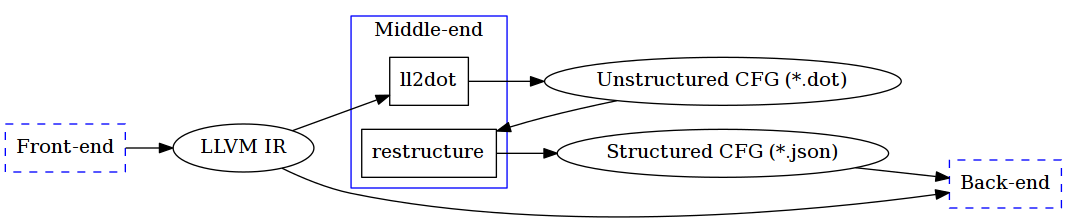
\includegraphics[width=\textwidth]{inc/middle-end.png}
		\caption{foo}
		\label{fig:middle-end}
	\end{center}
\end{figure}

% --- [ Subsubsections ] -------------------------------------------------------

% ~~~ [ Control Flow Graph Generation ] ~~~~~~~~~~~~~~~~~~~~~~~~~~~~~~~~~~~~~~~~

\subsubsection{Control Flow Graph Generation}
\label{sec:design_control_flow_graph_generation}

The control flow graph generation component generates a CFG for each function of a given LLVM IR assembly file. As described in section \ref{sec:lit_review_llvm_ir}, a function definition in LLVM IR consists of a set of basic blocks; and a basic block consists of zero or more non-branching instructions followed by a terminating instruction (such as \texttt{br} or \texttt{ret}) which changes the control flow. Therefore, the control flow graph generation component may focus on analysing the last instruction of each basic block, as they will determine the control flow.

To generate the CFG of a given function, a directed graph is created and populated with one node per basic block, and with zero or more directed edges between the nodes of the graph. The node names are determined by the basic block labels, and the directed edges are determined by the terminating instructions, as illustrated in figure \ref{fig:cfg_gen_example}.

\begin{figure}[htbp]
	\centering
	\begin{subfigure}[ht]{0.54\textwidth}
		\lstinputlisting[language=llvm, style=nasm, tabsize=2]{inc/cfg_gen_example.ll}
	\end{subfigure}
	\enskip
	\begin{subfigure}[ht]{0.22\textwidth}
		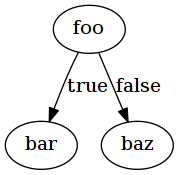
\includegraphics[width=\textwidth]{inc/cfg_gen_example.png}
	\end{subfigure}
	\caption{The return instructions of basic block \texttt{bar} and \texttt{baz} produces no directed edges, while the conditional branch instruction of basic block \texttt{foo} produces two directed edges, one for each target branch (i.e. \texttt{bar} and \texttt{baz}).}
	\label{fig:cfg_gen_example}
\end{figure}


The \texttt{ll2dot} tool generates CFGs from LLVM IR in the DOT file format, which is a well-defined textual representation of graphs used by the Graphviz project. One benefit of expressing CFGs in this format, is that the existing Graphviz tools may be facilitated to produce image representations of the CFGs; as demonstrated in appendix \ref{app:control_flow_graph_generation_example}.

% ~~~ [ Control Flow Analysis ] ~~~~~~~~~~~~~~~~~~~~~~~~~~~~~~~~~~~~~~~~~~~~~~~~

\subsubsection{Control Flow Analysis}
\label{sec:design_control_flow_analysis}

The key idea behind the control flow analysis (see section \ref{sec:control_flow_analysis}), is that high-level control flow primitives may be represented using directed graphs. The problem of structuring low-level code may therefore be rephrased as the problem of identifying subgraphs (e.g. the graph representation of high-level control flow primitives) in graphs (e.g. the CFGs of low-level code) without considering node names, as illustrated in figure \ref{fig:representation_and_identification_of_primitive}. This problem is generally referred to as \textit{subgraph isomorphism search} and has been well studied \cite{subgraph_isomorphism_algorithms}. Rephrasing the problem in this manner aligns with the design principle of giving each component access to the least amount of information required to successfully accomplish its task. The control flow analysis component is only given access to control flow information (e.g. CFGs), and is oblivious of the underlying LLVM IR. This enables the component to be reused as-is when analyzing the control flow of other languages, such as REIL.

\begin{figure}[htbp]
	\centering
	\begin{subfigure}[ht]{0.10\textwidth}
		\lstinputlisting[language=go, style=go, breaklines=false, numbers=none]{poster/inc/if.c}
		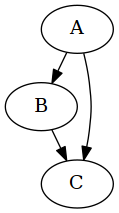
\includegraphics[width=\textwidth]{poster/inc/if.png}
	\end{subfigure}
	\enskip
	\begin{subfigure}[ht]{0.18\textwidth}
		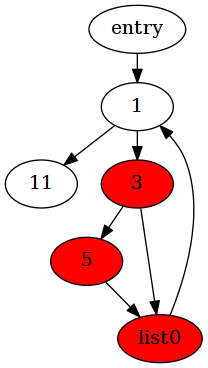
\includegraphics[width=\textwidth]{poster/inc/foo.png}
	\end{subfigure}
	\caption{The left side contains the pseudo-code (top left) and graph representation (bottom left) of an if-statement; if \texttt{A} is true then do \texttt{B} followed by \texttt{C}, otherwise do \texttt{C}. The right side highlights (in red) an identified isomorphism of the if-statement's graph representation, in the CFG of the \texttt{main} function presented in appendix \ref{app:clang_example}.}
	\label{fig:representation_and_identification_of_primitive}
\end{figure}

The \texttt{restructure} tool uses subgraph isomorphism search algorithms to locate isomorphisms of the graph representations of high-level control flow primitives in the CFG of a given function. The CFG is simplified by recursively replacing the identified subgraphs with single nodes until the entire CFG has been reduced into a single node; a step-by-step demonstration of which is presented in appendix \ref{app:control_flow_analysis_example}. By recoding the node names of the identified subgraph isomorphisms and the name of their corresponding high-level control flow primitives, a structured CFG may be produced in which all nodes are known to belong to a high-level control flow primitive; as demonstrated in appendix \ref{app:restructure_example}.

The pseudo-code and graph representations of the supported high-level control flow primitives are presented in figure \ref{fig:graph_representations} of section \ref{sec:control_flow_analysis}. Should the control flow analysis fail to reduce a CFG into a single node, the CFG is considered irreducible with regards to the supported high-level control flow primitives, in which case a structured CFG cannot be produced.

The \texttt{restructure} tool relies entirely on subgraph isomorphism search to produce structured CFGs (in JSON format) from unstructured CFGs (in the DOT file format). The supported high-level control flow primitives are defined using DOT files, thus promoting a data-driven design which separates data regarding the primitives from the implementation of the \texttt{restructure} tool. A major benefit with this approach is that the \texttt{restructure} tool may search for any high-level control flow primitive that can be expressed in the DOT file format, without any modification to the source code.

One limitation with this approach is that it does not support graph representations of high-level control flow primitives with a variable number of nodes, as they cannot be described in the DOT file format. For this reason, the \texttt{restructure} tool does not support the recovery of n-way conditionals (e.g. \texttt{switch}-statements). Furthermore, the current design enforces a single-entry/single-exit invariant on the graph representation of high-level control flow primitives. This prevents the recovery of infinite loops, as their graph representation has no exit node. A discussion of how these issues may be mitigated in the future is provided in section \ref{sec:design_validation}.

